\chapter{Introduction}
\label{chap:introduction}

Transport Layer Security (TLS) Protocol is a cryptographic protocol that provides secure transport connection between applications over a computer network, e.g. web server and web browser. 
 Using TLS prevents eavesdropping, tampering and message forgery. It provides privacy and data integrity between communicating applications. The protocol secures transmitted data using encryption. Secure communication with Authenticated Key Etablishment (AKE) and secure channel with Authenticated Encryption (AE). 
 Using Datagram TLS (DTLS) the stateless TLS is feasible. It offers server and, optionally, client authentication to confirm the identities of parties involved in the communication. 
 
 Further, the integrity check value implemented in the protocol provides integrity for the transferred data. TLS is also known or referred to as Secure Socket Layer (SSL), its predecessor. 
 
To use TLS all communicators must know that the other is supporting TLS.

TLS 1.2 was defined in RFC 5246 in August 2008. Its successor TLS 1.3 is defined in RFC 8446 in August 2018.
 \cite{RFC5246}

\section{Structure of the TLS Protocol}
\label{sec:stucture}

The TLS Protocol is layered between the Application layer and the TCP/IP layer according to the Internet Model (or between Session and Transport layers according to the OSI Model), where it can secure and then send application data to the transport layer \cite{ms:overview}. Thus it can support multiple application layer protocols, such as HTTP, FTP, SMTP, POP3. The protocols using TLS become respectively HTTPS, FTPS, SMTPS, POP3S and so on.

The TLS Protocol can be split into two layers. The lower layer of the TLS is the Record Protocol. The upper layer is the Handshake layer which consists of the following protocols: Handshake Protocol, ChangeCipherSpec Protocol and Alert Protocol. Figure \ref{fig:tls_structure} illustrates the structure of the TLS Protocol. 


\begin{figure}[H]
	\centering
		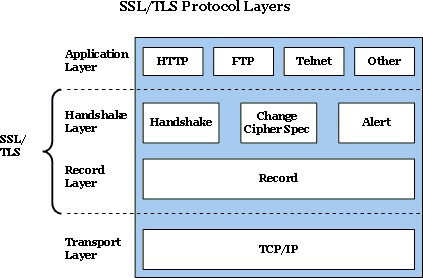
\includegraphics[scale=1]{images/tls_structure.jpg}
	\caption{TLS 1.2 Protocols Structure \cite{ms:overview}}
	\label{fig:tls_structure}
\end{figure}


\section{Record Protocol}
\label{sec:record_protocol}

The connection of two independent channels is established through the TLS Handshake, from the client to the server and in the other direction from the server to the client. The Record Protocol is responsible for the data protection on these channels using the authenticated encryption scheme.\\
The responsibilities of the Record Protocol are:
\begin{itemize}
	\item fragmentation
	\item compression
	\item application of MAC and encryption
	\item transmisson 
\end{itemize}
But the tasks/responsiblies depend also on the parameters of the keys, namely how the keys were set during the handshake protocol. \\

The processing of data is illustrated and described below:      

\begin{figure}[H]
	\centering
		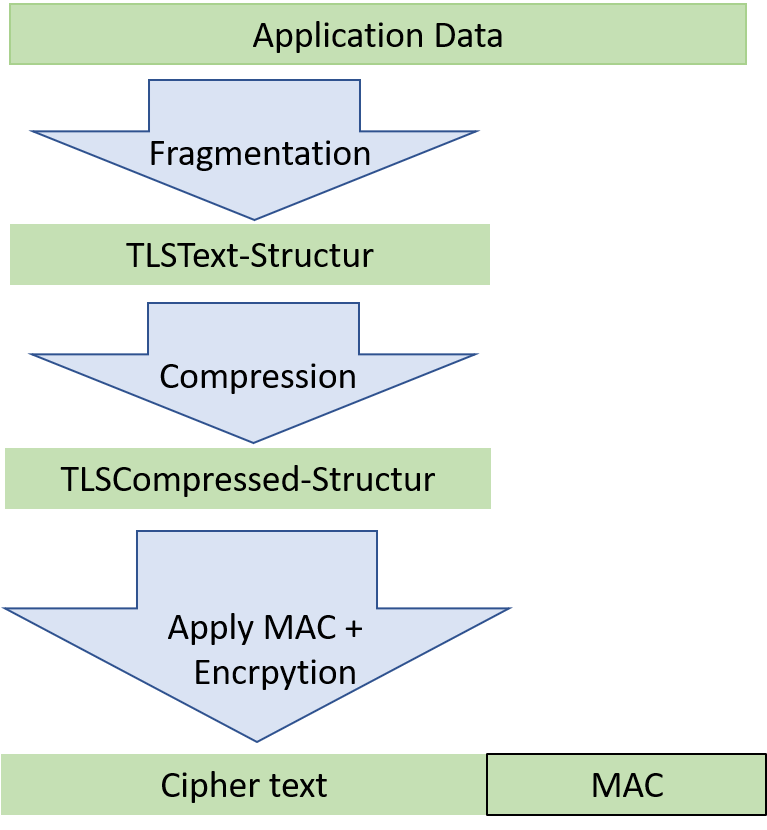
\includegraphics[scale=0.5]{images/tls_recordprotocol.png}
	\caption{TLS Record Protocol}
	\label{fig:tls_recordprotocol}
\end{figure}

First the Record Protocol layer receives the data from the application layer. Then it fragments the data to a size appropriate for the cryptographic algorithm. 
The next step is the compression, which is done if specified. The compression algorithm would then be defined in the current session state and would translate the date to a TLSCompressed structure.
 
Subsequently the message authentication code over the compressed data would be computed.
To ensure that the data were not altered during the transmission, the MAC value is added. So the receiver can check if the incoming MAC value and the computed one 
match. Thus, the integrity and confidentiality are ensured.

As a hint, the first handshake is neither secured by a MAC nor encrypted. Because this is the initial value for the keys, it is how they are first set. After the first handshake these parameters are set and therefore secured and encrypted.
\cite{ms:Record}